\documentclass{bioinfo}
\copyrightyear{2017} \pubyear{2017}
\usepackage{float}

\access{Advance Access Publication Date: Day Month Year}
\appnotes{Application Note}

\begin{document}
\firstpage{1}

\title[short Title]{GPU accelerated KMC2}
\author[]{Huiren Li\,$^{\text{\sfb 1,}*}$, Anand Ramachandran\,$^{\text{\sfb 1}}$ and
Deming Chen\,$^{\text{\sfb 1,}*}$}
\address{$^{\text{\sf 1}}$Department of Electrical and Computer Engineering, University of
Illinois at Urbana-Champaign, Urbana, IL 61801, USA}

\corresp{}

\history{Received on XXXXX; revised on XXXXX; accepted on XXXXX}

\editor{Associate Editor: XXXXXXX}

\abstract{\textbf{Motivation:} K-mer counting is a popular pre-processing step in many
bioinforamtic algorithms. KMC2 is one of the most popular tools for k-mer counting. In
this work, we leverage the computation power of GPU to accelerate KMC2. Our goal is to
reduce the overall runtime of many genome analysis tasks that use K-mer counting as an
essential step.\\
\textbf{Results:} We achieved 3.8x speedup using one GTX 1080 Ti with one CPU (Xeon
E5-2603)
thread and 5.2x speedup using one GPU with four CPU threads over a single thread CPU.\\
\textbf{Contact:} \href{dchen@illinois.edu}{dchen@illinois.edu}\\}

\maketitle

\section{Introduction}

K-mer counting refers to counting the frequencies of all k-length strings in a collection
of sequencing reads.
K-mer counting is a fundamental step for many bioinformatic algorithms, such as BLESS 2
\citep{Heo16} and Gerbil \citep{Mar17}.

The idea behind k-mer counting is very simple. The most naive way is to count k-mers using
brutal force, such as building a local histogram to count the frequencies of all k-mers.
This method could work if we have thousands of genome reads. Only, in real life, we would
have millions of genome reads to process. With a naive algorithm, k-mer counting can take
a large amount of memory and take a long time to run.

Different k-mer counting algorithms have been developed.
KMC2 \citep{Seb14} is a one of the most popular k-mer counting tools. KMC2 is designed to
be memory frugal and fast while some other k-mer counting tools would use tens of
gigabytes of memory like Jellyfish \citep{Mar11} and BFCounter \citep{Mel11}.
The memory frugality of KMC2 is the most important reason why we chose to implement this
particular algorithm on GPU.

Even with tools like KMC2, k-mer counting would still take a substantial amount of time to
process. The original KMC2 was implemented purely using CPU.
In this work, we would like to exploit the computation power of GPU and further optimize
the running time of KMC2. We developed a memory-efficient GPU implementation of KMC2 for
acceleration because GPU usually does not have a very large memory.
We achieved a substantial speedup over the original CPU implementation while maintaining a
small memory footprint.
%\enlargethispage{12pt}

\section{Approach}
There are two key concepts behind KMC2: signature and super k-mer.
A signature is lexicographically the smallest m-mer where m is smaller or equal to k.
Another constraint for a signature is that it cannot contain substring sequence AA and it
does not start with AAA or ACA.
A super k-mer is formed by consecutive k-mers which share the same signature.

KMC2 is a disk based k-mer counting algorithm. It includes two major stages, a
distribution stage and a sorting stage. There is also a pre-processing stage to calculate
the signature map for distribution of super k-mers. By dividing the super k-mers into
different bins, KMC2 is capable of maintaining a small memory footprint while collecting
statistics of all the k-mers.
The idea of signature is introduced to balance the number of super k-mers stored in each
bin and it is used to extract super k-mers from the sequencing reads and distribute them
to their corresponding bins.

The first stage is to extract super k-mers from the sequencing reads and distribute them
to their corresponding bins on the disk according to the signature map.
Super k-mers are used in this stage instead of naive k-mers to reduce disk footprint.
In our implementation, we have a total of 512 bins in the first stage.

In the second stage, we process the bins one at a time. For each bin, we expand the super
k-mers stored in the bin. Then we sort the expanded k-mers, collect the statistics of it
and store the result.


\begin{figure*}[t]
	\centering
	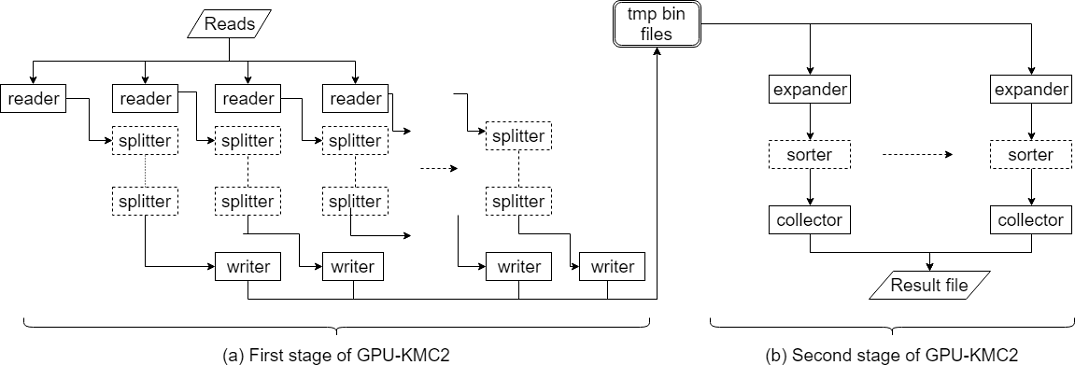
\includegraphics[scale=0.5]{kmc2.png}
	\caption{Overview of GPU acclerated KMC2. Rectangles with dotted lines are processes
	that are parallelized using CUDA.}\label{fig:01}
\end{figure*}
\newpage
\begin{methods}
\section{Methods}
\enlargethispage{6pt}
Our GPU accelerated KMC2 is parallelized using CUDA and OpenMP. Currently, we are only
using a single GPU to perform the computation and it could be further accelerated using
multiple GPUs.

The overall algorithm is shown in Figure~1\vphantom{\ref{fig:01}}.
In the first stage, the host will read the sequencing reads from the fastq file and store
it in a buffer.
When enough reads are stored in the buffer, it will pass the sequencing reads to the GPU
side for processing.
Each GPU thread is a splitter responsible for one sequencing read. The splitters will
split the super k-mers from the reads and store them in the buffer in gloabl memory on
the device.
After the result is copied back to the host, it will be dumped into the temporary bin
files.

There are two key challenges in exporting KMC2 to GPU.
The first limitation is the limitation of memory on GPU.
We have to identify the limitations of GPU computation and utilize all the memory we have
in GPU.
The second challenge is that reading fastq file is time consuming and it is essential to
hide the latency of file IO in our implementation.

We have two options to implement the buffer for the bins. We could
have a global buffer shared by all threads or each thread could have its own buffer.
Using the global buffer is more memory efficient but it requires a lock for every bin in
the buffer.
Dealing with locks on the device side among different versions of CUDA is challenging but
it could be resolved by the keyword "volatile" together with atomic operations.
Although giving each thread its own buffer space avoids the pain of dealing with locks in
CUDA, it limits the number of reads we could process during each batch.
The later method turns out to be worse because of the large memory overhead it introduces.
Moreover, since we would process fewer reads during each batch of work, we have to call
cudaMemcpy more times which also introduces a larger overhead.

To minimize the running time of the first stage, we maximized the overlap between host and
device computation.
The readers on the host CPU are responsible for fetching reads from the fastq file.
The splitters on the GPU device will process the reads and split the reads into different
 bins.
At last, the writers on the host CPU will store the result of splitters onto the disk.
The readers and writers are serial work and cannot be accelerated through GPU.
Therefore, the readers and writers are implemented on the CPU side and we tried to 
maximize the overlap between CPU and GPU computation.
As shown in Figure~1\vphantom{\ref{fig:01}}, when the kernels for splitters are running on
the device side, the host first writes the result of the previous batch to the disk if
that batch exits and then prepares the reads for the next batch.
Therefore, the idle time of the device is minimized.
Figure~1\vphantom{\ref{fig:01}} shows the collaboration between GPU and CPU in
the first stage.

The other technique we used is dividing the kernels into streams.
K-mer counting is a memory intense process. This means the time spent on copying data
between host and device is not negligible.
Currently, the kernels are divided into four streams to overlay the kernel executions and
cudaMemcpy's to hide the memory latency.
If we are only using a single stream, at the beginning of each batch, we have to wait for
cudaMemcpy to copy all the reads from host to device.
At the end of each batch, we have to wait for cudaMemcpy to copy all the results from
device to host.
The kernel would be idle during this process.
By dividing the kernel into four streams, we only pays for one fourth of the overhead
because each cudaMemcpy needs to copy one fourth of the previous workload.
After the first cudaMemcpyHostToDevice finishes, the kernel for the first stream can be
launched and cudaMemcpyHostToDeice for the second stream can be launched concurrently.

There are three major steps in the second stage.
The first one is expander; it is used to pre-process the super k-mers. The second step is
a sorter to sort the result from the first step. The third step is a collector to collect
statistics from the sorted results and store it in the result file.

The expander and collector are serialized work. This makes their performance on the GPU
non-ideal.
Therefore, instead of moving the computation to the device side, the expander and
collector are implemented on the host side.
The sorter uses radix sort which can be easily parallelized on GPU.
Therefore, a collaborative processing with both GPU and CPU is more efficient.
We used radix sort implemented in Thrust \citep{Jared} provided by NVIDIA to perform the sorting in the sorters on GPU.

However, simply using the Thrust to parallelize the sorters didn't give us a satisfactory
speedup.
This is caused by the serialization between the expander and collector.
The GPU remains idle when it is waiting for the data for the expander and it could not
begin to process the data from the next bin until the previous bin's collector finishes
its job.

There is still one more level of parallelism to explore in KMC2.
Since each bin is independent from each other, we can use OpenMP to process multiple bins
at the same time.
In our implementation, we used four OpenMP threads to process four bins simultaneously.
This allows us to prepare data of four different bins at the same time and reduce the 
amount of time that the GPU sits idle.
The drawback of using OpenMP together with Thrust is that only one sorting kernel can be
launched at a time because Thrust doesn't allow concurrent kernel launching. CPU threads
could stay idle while waiting for other thread to finish sorter computation on GPU and
this creates additional latency.
\newline

\end{methods}

\section{Results and Conclusion}
In order to evaluate the performance of the GPU acceleration for KMC2, we tested our
implementation against the original KMC2 \citep{Seb14}.

All experiments are done using Xeon E5-2603 v2 CPU and GeForce GTX 1080 Ti.
\begin{table}[H]
\processtable{K-mer counting results, speedup is calculated using GPU KMC2 with one CPU thread
\label{Tab:01}} {\begin{tabular}{@{}lllll@{}}\toprule
& first & second & total & our\\\
& stage(s) & stage(s) & runtime(s) & speedup\\\midrule
k-mer length=40\\\
GPU KMC2 (1 thread) & 23 & 85 & 108 & N/A\\
GPU KMC2 (4 threads) & 23 & 51 & 74 & 0.7x\\\
DSK (1 thread) & N/A & N/A & 866 & 8.0x\\\
DSK (4 threads) & N/A & N/A & 224 & 2.1x\\\
JellyFish2 (1 thread) & N/A & N/A & 1072 & 9.9x\\\
JellyFish2 (4 threads) & N/A & N/A & 320 & 3.0x\\\
KMC2 (1 thread) & 127 & 307 & 435 & 4.0x\\\
KMC2 (4 threads) & 62 & 85 & 148 & 1.4x\\\
k-mer length=50\\\
GPU KMC2 (1 thread) & 29 & 86 & 115 & N/A\\\
GPU KMC2 (4 thread) & 29 & 58 & 87 & 0.8x\\\
KMC2 (1 thread) & 101 & 298 & 400 & 3.5x\\\
KMC2 (4 threads) & 42 & 80 & 123 & 1.1x\\\botrule
\end{tabular}}{}
\end{table}

The testing is done using 35249162 mouse genomes whose read length equals to 100.
The results are summarized in Table~\ref{Tab:01}.

Overall, the GPU implementation of KMC2 achieved a 3.8x speedup over single thread CPU
version while using one CPU thread and achieved a 5.2x speedup while using four CPU
threads.

Note that we achieved a 4.5x speedup in the first stage disregard the number of CPU
threads we used because we are not using OpenMP in the first stage.
Moreover, the speedup we got using GPU with 4 CPU threads is not very significant.
The reason is that the sorters are not parallelized by OpenMP. Even multiple CPU threads
are running at the time, only one sorter kernel could be launched.
There is a large overhead in this process due to the serialized cudaMemcpy's and kernel
launched. Therefore, it prevented further performance gain.

We also compared the performance of our implementation against two other popular k-mer
counting tools, JellyFish 2 and DSK \citep{Rizk13}.
We achieved 8.02x speed up over DSK and 9.9x speed up over JellyFish2 if only one CPU
thread is used.

\begin{thebibliography}{}

\bibitem[Deorowicz {\it et~al}., 2014]{Seb14}
Deorowicz,S.,Kokot,M.,Grabowski,S.,Debudaj-Grabysz,S. (2014). KMC 2: Fast and resource-
frugal k-mer counting, {\it Bioinformatics}, {\bf 00}, 1-21.

\bibitem[Heo {\it et~al}., 2016]{Heo16}
Heo,Y., Ramachandran,A., Hwu,W., Ma,J., Chen,D. (2016). BLESS 2: accurate, memory-
efficient and fast error correction method, {\it Bioinformatics}, {\bf 146}.

\bibitem[Jared {\it et~al}., 2015]{Jared}
Jared H., Nathan B. (2015). Thrust:https://thrust.github.io/

\bibitem[Marcais {\it et~al}., 2011]{Mar11}
Marcais,G., Kingsford,C. (2011).  A fast, lock-free approach for effi-
cient parallel counting of occurrences of k-mers, {\it Bioinformatics}, {\bf 146},
764-770.

\bibitem[Marius {\it et~al}., 2017]{Mar17}
Marius, E., Steffen, R., Matthias, M. (2017). Gerbil: a fast and memory-efficient k-mer
counter with GPU-support, {\it Algorithms for Molecular Biology}.

\bibitem[Melsted {\it et~al}., 2011]{Mel11}
Melsted,P., Pritchard,J.K. (2011). Efficient counting of k-mers in DNA sequences
using a bloom filter. {\it BMC Bioinformatics}, {\bf 12}, 333.

\bibitem[Rizk {\it et~al}., 2013]{Rizk13}
Rizk, G., Lavenier, D., Chikhi, R. (2013). DSK: k-mer counting with very low memory usage.
{\it BMC Bioinformatics}, {\bf 29}, 652-653.

\end{thebibliography}
\end{document}
